% Every reported number traces to results/*.txt in the code repository,
% https://github.com/prakharg55/cue_reliance (see analysis/check_numbers.py).
\documentclass[11pt]{article}
\usepackage[final]{acl}
\usepackage{times}
\usepackage{latexsym}
\usepackage[T1]{fontenc}
\usepackage[utf8]{inputenc}
% \usepackage{microtype} % broken with equation env on cluster texlive; re-enable for camera-ready
% \usepackage{inconsolata} % not installed on cluster; optional per template
\usepackage{graphicx}
\usepackage{booktabs}
\usepackage{amsmath}
\usepackage{amssymb}

\newcommand{\cued}{\ensuremath{\Delta_{\mathrm{cue}}}}

\title{Ask the Model: Counterfactual Cue Reliance Predicts\\
Worst-Group Failure and Targets Repair}

\author{
\textbf{Prakhar Gupta\textsuperscript{1,2}}\thanks{Email: \texttt{prakharg@umich.edu}.} \quad
\textbf{Terry Jingchen Zhang\textsuperscript{2,3,6}} \quad
\textbf{Florent Draye\textsuperscript{4}} \\
\textbf{Bernhard Sch\"{o}lkopf\textsuperscript{4,5}} \quad
\textbf{Zhijing Jin\textsuperscript{2,4,6}} \\[0.15em]
\textsuperscript{1}University of Michigan \quad
\textsuperscript{2}Jinesis Lab, University of Toronto \& Vector Institute\\
\textsuperscript{3}University of Oxford \quad \textsuperscript{4}Max-Planck Institute for Intelligent Systems, T\"{u}bingen, Germany \\
\textsuperscript{5}ELLIS Institute T\"{u}bingen \quad
\textsuperscript{6}EuroSafeAI
}

\begin{document}
\maketitle

\begin{abstract}
Fine-tuned models can rely on shortcut cues that correlate with labels during
training but mislead on some inputs. We ask whether a finished model's behavior
reveals how much it relies on such a cue. Given a suspected cue, we measure
counterfactual cue reliance, \cued{}, by editing the cue and measuring the
change in the model's decision score. This requires no group labels, training
data, or knowledge of the training recipe. We test 486 fine-tuned language models on CivilComments and Bias-in-Bios while
varying the training cue--label correlation. Across 180 models in 10 main
task--model settings, higher \cued{} predicts lower worst-group accuracy. In a
separate high-seed analysis, \cued{} predicts at held-out correlation levels,
where linear extrapolation from the assigned correlation performs worse than
predicting the mean. Capability and placebo-edit controls show that neither model quality nor
generic edit sensitivity explains the result. \cued{} also provides
signal for prioritizing concept-erasure repair. Exact control shows that most of the predictive signal comes from differences
across correlation levels. Within a
fixed recipe, the relationship across random seeds is small and not robust.
\end{abstract}

\section{Introduction}

\begin{figure*}[t]
\centering
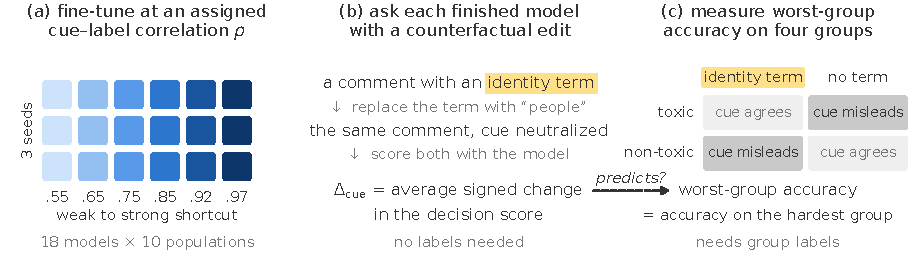
\includegraphics[width=0.97\textwidth]{fig_overview.pdf}
\caption{\textbf{Overview.} (a) Each of the 10 main populations has 18 LMs fine-tuned at six assigned cue--label correlations $\rho$. (b) \cued{} is the average signed change in the decision score after a counterfactual cue edit. (c) Worst-group accuracy is the outcome it should predict. Panels (b) and (c) show CivilComments, and Figure~\ref{fig:hero} reports the test.}
\label{fig:concept}
\end{figure*}

Recent work in mechanistic interpretability has argued for a more pragmatic,
action-oriented standard, where methods are evaluated by whether they support
concrete empirical tasks and interventions
\citep{nanda2025pragmatic,orgad2026actionable}. One natural test is whether a
measurement taken from a finished model can predict a downstream failure that
matters and help decide what to do about it.

Fine-tuned models provide a useful setting for this question because they can
rely on shortcut cues. These are features that correlate with the label during
training but become misleading on some inputs \citep{geirhos2020shortcut}. For example, if identity terms co-occur with toxic labels during training, a
toxicity classifier may learn to read an identity mention itself as evidence of
toxicity. It then does worse on non-toxic comments that mention an identity
\citep{borkan2019nuanced,koh2021wilds}. Our question is whether the finished
model itself can tell us how much it relies on such a shortcut.

We ask the model directly (Fig.~\ref{fig:concept}). Given held-out inputs containing a suspected cue, we
counterfactually edit the cue and measure the resulting change in the model's
decision score. A larger average shift in the cue-consistent direction indicates
greater reliance. For a classifier with decision score $s(x)$ and edited input
$\tilde{x}$, we define counterfactual cue reliance as
\begin{equation}
\cued \;=\; \mathbb{E}_{x}\!\left[\,s(x)-s(\tilde{x})\,\right].
\label{eq:cued}
\end{equation}
Once the cue and edit are specified, \cued{} requires no group labels, no access
to training data, and no knowledge of the training recipe. Counterfactual edits and model-reliance measurements are both well established
\citep{garg2019ctf,prabhakaran2019perturbation,kiritchenko2018eec,
fisher2019models}. We test whether this simple measurement, taken on its own from a finished model, predicts meaningful downstream failure,
transfers to unseen training-correlation levels, and gives useful information
for repair.

To test this, we train 486 decoder LMs on two shortcut-prone tasks while
deliberately varying the training cue--label correlation
$\rho \in \{0.55,\dots,0.97\}$ and random seed. The tasks are CivilComments
toxicity classification with an identity-term cue
\citep{borkan2019nuanced,koh2021wilds} and Bias-in-Bios profession
classification with a gendered-word cue \citep{dearteaga2019bios}. Because
$\rho$ is experimentally assigned, we can directly compare what the finished
model reveals with simple extrapolation from the assigned training correlation.

\begin{figure*}[t]
\centering
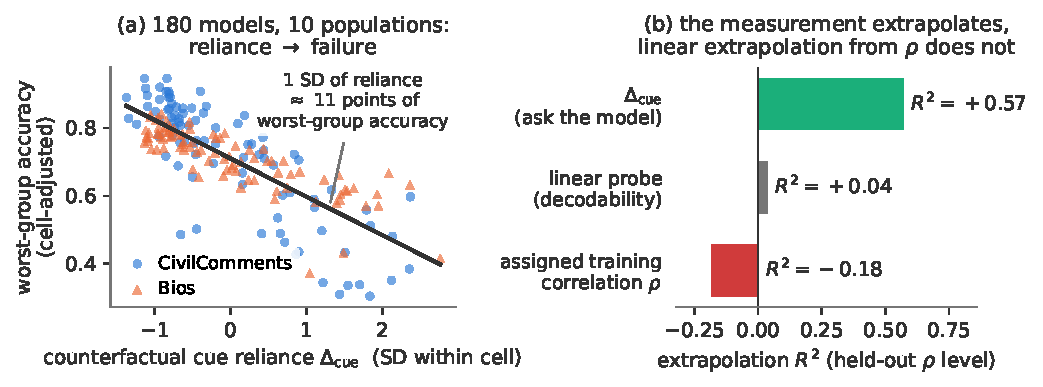
\includegraphics[width=0.92\textwidth]{fig_hero.pdf}
\caption{\textbf{Measured cue reliance predicts worst-group failure across training-correlation levels.} (a)~$\beta{=}{-}0.113$ per within-cell SD of \cued{}, partial $R^2{=}0.63$ beyond population identity. This pooled relationship includes the across-level effect. Section~\ref{sec:exact} isolates the within-level estimate. (b)~Each predictor is fit on two $\rho$ levels and predicts models at the held-out third. \cued{} transfers, and linear extrapolation from $\rho$ does worse than predicting the mean.}
\label{fig:hero}
\end{figure*}

\paragraph{Contributions.}
We make three main findings:
\begin{itemize}
    \setlength{\itemsep}{8pt}
    \setlength{\parskip}{0pt}
    \setlength{\parsep}{0pt}

    \item \textbf{Cue reliance predicts shortcut failure.}
    Across 180 models in 10 task--model settings, higher \cued{} predicts lower
    worst-group accuracy. The prediction also holds at held-out training-correlation levels in a separate high-seed analysis. There, linear extrapolation from the assigned correlation performs worse than predicting the mean. Neither general model quality nor generic edit sensitivity explains the result (\S\ref{sec:prediction}--\ref{sec:validity}).

    \item \textbf{Cue reliance provides signal for repair.}
    We compare five post-hoc repairs under one protocol. LEACE improves mean
    worst-group accuracy in all six settings tested, and hard directional
    ablation can be harmful. \cued{} also provides signal for choosing which
    models to repair with LEACE (\S\ref{sec:repair}).

    \item \textbf{Most of the predictive signal is across correlation levels.}
    Treating the discrete assigned correlation as a linear control initially
    made \cued{} appear predictive beyond the training correlation. Exact control removes that apparent effect. Among models trained with
    the same recipe but different random seeds, the remaining relationship is
    small and statistically fragile (\S\ref{sec:exact}).
\end{itemize}

These results validate \cued{} as a simple per-model audit. In the controlled
populations we study, measuring what a finished model uses can tell us more
about shortcut failure than extrapolating from the assigned training
correlation.


\section{Related Work}
\label{sec:related}

Our question connects work on shortcut measurement, cross-model prediction, and
robust repair.

\paragraph{Measuring reliance.}
Counterfactual edits are widely used to test whether predictions depend on
sensitive or spurious features
\citep{garg2019ctf,prabhakaran2019perturbation,veitch2021counterfactual}.
\citet{guardrail2026shortcuts} identify token-level shortcuts from a converged
model and mitigate them at deployment time, while \citet{ravuru2026unmask}
discover and causally verify text shortcuts for annotation-free debiasing. Related work also studies cue reliance through hidden-state bias
directions and probe-based representation entanglement
\citep{gupta2026alignment,entangle2026probe}, and its mitigation via consistency training \citep{chua2025biasaugmentedconsistencytrainingreduces,imran2026consistencytrainingmitigatingobfuscation}. We ask a different question, namely whether a reliance score read off a
finished model predicts worst-group accuracy across independently trained
models and at held-out assigned cue--label correlations. The question is open
because model-side bias measurements do not necessarily predict downstream
bias
\citep{goldfarbtarrant2021intrinsic,cao2022intrinsic}.

\paragraph{Predicting robustness across models.}
Identically trained models can generalize differently
\citep{mccoy2020feather,damour2020underspecification}, and prior work asks
whether model-side measurements predict generalization across model populations
\citep{jiang2020fantastic,li2026interpretation}. Such comparisons can be driven
by the design factors used to generate the population
\citep{dziugaite2020search}, while in-distribution accuracy can itself predict
OOD accuracy \citep{miller2021accuracyline}. Other work predicts per-example OOD behavior from internal causal features
\citep{huang2025internal}. We assign the cue--label correlation directly and
test prediction at held-out levels of that assignment.

\paragraph{Repair.}
Worst-group robustness and post-hoc repairs are well studied
\citep{sagawa2020groupdro,liu2021jtt,kirichenko2023dfr,qiu2023afr,
belrose2023leace}. Model-side measurements can guide selective debiasing,
steering, and predictions of fine-tuning biases
\citep{kuzmin2025selective,steering2026predicting,lovering2021predicting},
while localization does not reliably identify editing layers
\citep{hase2023localization}. We work at the model level and ask whether a pre-repair score can rank
independently trained models by how much they gain from the same repair. Concurrent work also studies repair-aware model selection using group-annotated
validation performance \citep{wang2026prome}. Our reliance score needs no group labels.


\section{Methods}
\label{sec:design}

The design compares two ways of predicting failure. One measures the finished model. The other extrapolates from its assigned training correlation. That comparison
needs a population in which we assign the shortcut signal instead of inferring
it.

\paragraph{Populations.}
Each population \emph{cell} is one task--model pair. Within each cell, we vary
the assigned cue--label correlation
$\rho \in \{0.55,\allowbreak 0.65,\allowbreak 0.75,\allowbreak 0.85,\allowbreak 0.92,\allowbreak 0.97\}$ and random seed. This creates
models trained on the same task but exposed to shortcut signals of different
known strengths. The main analysis has 10 cells from two tasks crossed with five model
configurations: Qwen2.5-0.5B/1.5B, Pythia-410m/1.4b, and OLMo-2-1B.
Each cell contains six correlation levels and three seeds, giving 18 models per
cell and 180 models in total. A separate high-seed arm uses three cells
(Qwen-civil, Qwen-bios, and Pythia-civil) at
$\rho \in \{0.65,0.85,0.97\}$ with 15 seeds per stratum, giving 135 models. Throughout the paper, cell names without an explicit scale use the smallest
model in that family. Thus, Qwen refers to Qwen2.5-0.5B and Pythia refers to
Pythia-410m. Larger scales are named explicitly. Training sets contain 4{,}000 label-balanced examples and
realize the assigned $\rho$ exactly. Our main models use LoRA. Additional
full-fine-tuning and instruction-tuned-base arms test whether the result depends
on that choice. Across the main and auxiliary study arms, we train 486 models
in total. Full training details are in Appendix~\ref{app:config}.

\paragraph{Tasks and edits.}
CivilComments uses 32 unambiguous identity terms as the cue (Appendix~\ref{app:lexicons}), following the identity-term tradition of \citet{dixon2018measuring}. The edit replaces each identity term with ``people''. Bios uses gendered words, and the
edit swaps gender, applied only in the well-defined male$\rightarrow$female
direction. The two edits are different operations that measure the same target quantity
(Eq.~\ref{eq:cued}), and we verify in \S\ref{sec:validity} that what they
measure is cue-specific. Appendix~\ref{app:edits} audits both edits (coverage,
minimality, and the reason the bios swap is used in one direction only).

\paragraph{Measurement.}
Each input is scored with a fixed prompt. For CivilComments it is
\texttt{Comment:\ \{text\}}, a line break, \texttt{Question:\ Is this comment
toxic?}, a line break, and \texttt{Answer:}. For Bios the first two lines are
\texttt{Bio:\ \{text\}} and \texttt{Question:\ Is this person a professor or a
physician?}. The decision score $s(x)$ is the logit of the answer token \texttt{A} minus the
logit of \texttt{B} at the last position. \texttt{A} stands for toxic or
professor and \texttt{B} for non-toxic or physician. Each token has a leading
space and is looked up in the model's own tokenizer. \cued{} averages
$s(x)-s(\tilde{x})$ over 300 cue-containing texts drawn from the same held-out
pool as the evaluation groups. These texts never appear in training. They may
partially overlap the evaluation sample, and no labels are used in computing
\cued{}.

\paragraph{Outcome.}
We evaluate worst-group accuracy over the four
$(\text{label} \times \text{cue-present})$ groups. These groups separate cases
where the cue agrees with the label from those where it is misleading. For
Bios, every pooled bio contains gendered words and cue-present means the bio
is male, so the four groups are profession $\times$ gender. Worst-group
accuracy uses all four groups, while the edit is applied only in the
male$\rightarrow$female direction. We use a non-overlapping, deduplicated held-out split of 796--800 texts per group and
sample 400 per group for each evaluation. Our grouping is coarser than the
WILDS 16-cell definition \citep{koh2021wilds}, so the absolute numbers are not
comparable to that leaderboard.

\paragraph{Statistical protocol.}
Because $\rho$ is discrete and experimentally assigned, we control for it with
indicator variables rather than treating it as linear. Section~\ref{sec:exact}
shows why this matters. Population cells enter as fixed effects. The
within-recipe estimator was pre-specified as the equal-weighted mean of the
within-stratum slopes. Section~\ref{sec:exact} reports its robustness checks,
and Appendix~\ref{app:iv} gives the additional instrumental-variable analysis.

\section{\cued{} Predicts Worst-Group Failure}
\label{sec:prediction}

\begin{figure*}[t]
\centering
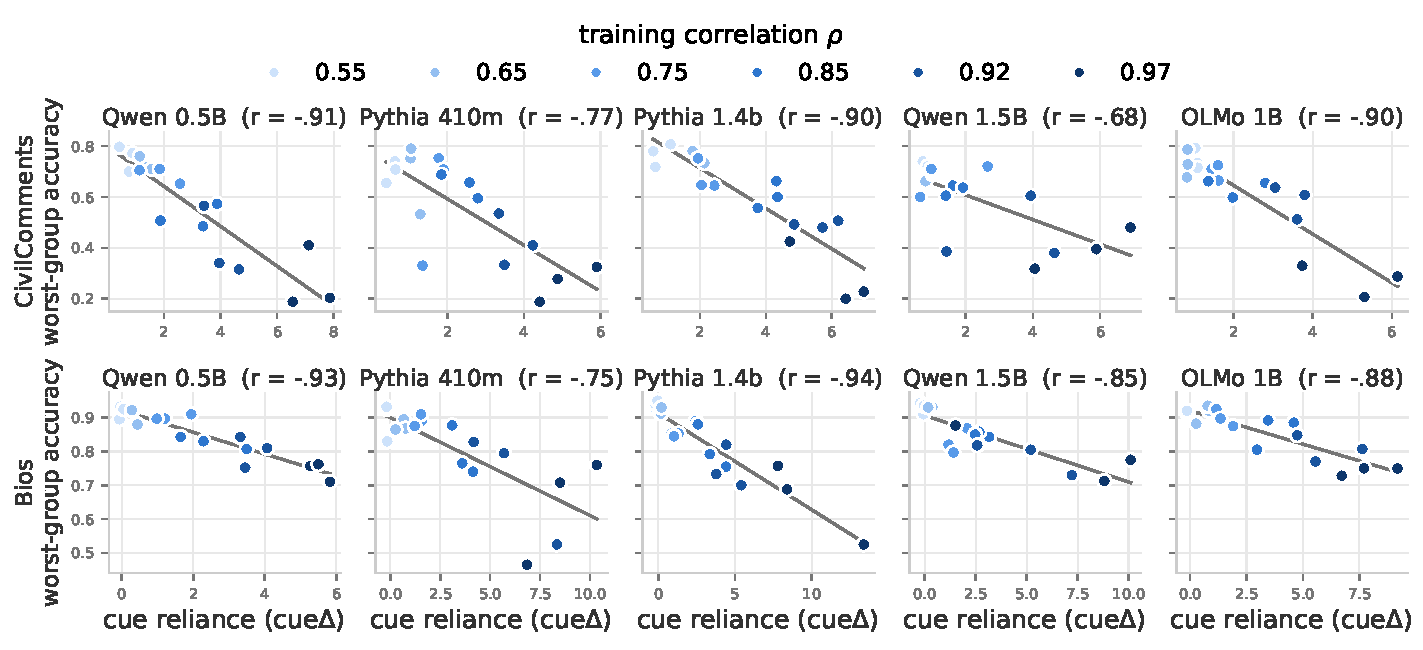
\includegraphics[width=0.96\textwidth]{fig_population.pdf}
\caption{\textbf{The relationship holds in every population cell.} Each panel is one cell, and each point is one fine-tuned model shaded by its assigned $\rho$ (per-cell $r$ from $-0.94$ to $-0.68$, all $p < 0.002$). Because the points span the $\rho$ levels, these correlations include the across-level effect (\S\ref{sec:exact}).}
\label{fig:population}
\end{figure*}

\paragraph{Within-population prediction.}
In every population we train, models that react more to the cue edit do
worse on the groups where the cue is misleading. The effect is large. When a
model's measured reliance is one standard deviation higher, its worst-group
accuracy is about eleven points lower ($\beta = -0.113$,
$p = 3.1{\times}10^{-38}$, $n{=}180$, Fig.~\ref{fig:hero}a). Knowing only
which population a model comes from explains less than half of the variance
($R^2 = 0.46$). Adding \cued{} raises this to $0.80$, a partial $R^2$ of
$0.63$. The relationship also holds in every cell on its own
(Fig.~\ref{fig:population}), so it is not an artifact of pooling.

\paragraph{Out-of-regime extrapolation.}
Within a designed population, both reliance and failure are consequences of
the assigned $\rho$. A sharper test is to predict a correlation level the
predictor has never seen. We fit the predictor on two $\rho$ levels
and predict models from the held-out third (high-seed arm, $n{=}135$, cell
fixed effects). \cued{} transfers to the held-out level, while simple extrapolation from the
assigned correlation does not (Fig.~\ref{fig:hero}b, Table~\ref{tab:oor}).
Extrapolating $\rho$ itself performs worse than predicting the mean
($R^2{=}{-}0.18$). The reason is that $\rho$'s effect on worst-group accuracy
is strongly nonlinear (\S\ref{sec:exact}), so a line fitted on two levels
misplaces the third. A nearest-level step extrapolation, the natural alternative with two observed levels, also performs worse than predicting the mean ($R^2{=}{-}0.14$). Because \cued{} is measured after training, it can reflect how strongly the finished model came to rely on the cue.
This result is mainly about placing models across correlation levels. \cued{} does not consistently rank individual models within a held-out
level (per-fold $R^2$ of $-0.85$, $+0.69$, and $+0.19$). We study fixed-recipe
ranking directly in \S\ref{sec:exact}.


\paragraph{Robustness to the fine-tuning setup.}
The relationship remains similar under full-parameter fine-tuning and under an
instruction-tuned base ($r = -0.905$ LoRA/base, $-0.897$ full FT,
$-0.907$ instruct, $n{=}18$ each).

\section{Validity Controls}
\label{sec:validity}

The prediction would be uninformative if \cued{} merely restated model
competence or generic sensitivity to edits. We test both alternatives directly.
Within our controlled populations, neither accounts for the result.

\paragraph{Capability control.}
In-distribution competence predicts robustness across models
\citep{miller2021accuracyline}. In our own attempt to extend this study to
public toxicity classifiers, capability explained nearly all of the variation
(Spearman $+0.98$, see Limitations). Overall accuracy is not a clean capability control within our population
because it already includes the worst group. We therefore build a control from
non-overlapping example sets. We predict
accuracy on the groups where the cue disagrees with the label from \cued{}
while controlling for accuracy on the groups where it agrees. On the 108 bios models that log all four groups, \cued{} still strongly
predicts accuracy on the harmed groups after this control
($\beta = -0.076$, $p = 8.0{\times}10^{-21}$), adding partial
$R^2 = +0.25$. The capability control itself adds no detectable predictive value
($p = 0.77$).

\begin{figure}[t]
\centering
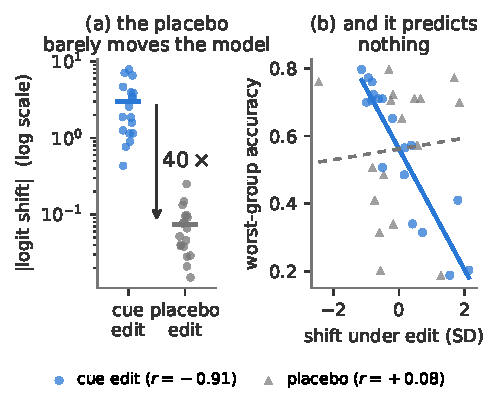
\includegraphics[width=0.9\columnwidth]{fig_placebo.pdf}
\caption{\textbf{Placebo edits barely move the model and predict nothing.} The same edit applied to 32 frequency-matched non-cue words shifts the decision score $40\times$ less (a). Across the same 18 models, the placebo shift does not track worst-group accuracy ($r{=}{+}0.08$), while \cued{} does ($r{=}{-}0.905$) (b).}
\label{fig:placebo}
\end{figure}

\paragraph{Placebo-edit control.}
We repeat the same procedure using 32 frequency-matched non-cue words. These
placebo edits move the model about $40\times$ less than the actual cue edits
and do not predict worst-group accuracy
($r{=}{+}0.08$ versus $r{=}{-}0.905$ for \cued{},
Fig.~\ref{fig:placebo}). So the measurement responds to the cue itself. Editing text in general does
not produce it.

\paragraph{Reliable measurement.}
Split-half reliability of \cued{} across models is $0.993$
(Spearman--Brown $0.996$, within-model SE $0.12$ vs.\ between-model SD
$2.32$). The small within-recipe effects below are therefore unlikely to be explained
by measurement noise alone.

\section{Repair: What Works, and for Whom}
\label{sec:repair}

A useful audit should predict failure and also say what to do about it.

\begin{table}[t]
\centering\small
\setlength{\tabcolsep}{4.2pt}
\begin{tabular}{lrrrrr}
\toprule
cell & ablate & prosp. & LEACE & DFR & AFR \\
\midrule
Qwen-civil   & $+.067$ & $+.056$ & $+.064$ & $+.180$ & $+.002$ \\
Pythia-civil & $-.262$ & $-.208$ & $+.111$ & $+.186$ & $+.048$ \\
OLMo-civil   & $-.185$ & $-.169$ & $+.079$ & $+.160$ & $+.020$ \\
Qwen-bios    & $+.043$ & $+.035$ & $+.028$ & $+.079$ & $+.003$ \\
Pythia-bios  & $+.039$ & $+.059$ & $+.060$ & $+.128$ & $+.051$ \\
OLMo-bios    & $+.049$ & $+.052$ & $+.038$ & $+.084$ & $+.024$ \\
\bottomrule
\end{tabular}
\caption{\textbf{LEACE improves mean worst-group accuracy in every cell, while hard ablation can be strongly harmful.} Mean change in worst-group accuracy ($n{=}18$/cell) for five post-hoc repairs: fixed-depth directional ablation, ablation at a prospectively selected layer, LEACE erasure, DFR-style group-balanced head refit, and AFR-style reweighting. Only DFR uses group labels.}
\label{tab:repair}
\end{table}

\paragraph{Five repairs, one protocol.}
Table~\ref{tab:repair} compares five repairs, and three patterns stand out.
First, LEACE improves mean worst-group accuracy in every cell. Second, hard
directional ablation is very harmful in the civil cells of two of three
families, and it gets worse with scale ($-0.385$ at Pythia-1.4b, $-0.344$ at
Qwen-1.5B). This matches known failure modes of subspace interventions,
namely damage to task-relevant features \citep{kumar2022probing} and
off-manifold artifacts \citep{makelov2023illusion}. Third, DFR is the strongest repair everywhere, but it needs group labels. Our variant refits on training data, since the held-out split is our only evaluation. This may overstate its performance relative to \citet{kirichenko2023dfr}. AFR,
which uses class labels but no group labels, is near zero. LEACE's worst-group gains do not come with large overall-accuracy losses. Post-LEACE overall accuracy stays within $0.03$ of label-dependent DFR's in
every cell. The cells where ablation is harmful also show large
overall-accuracy drops ($0.63$--$0.69$ vs.\ $0.77$--$0.79$ under LEACE in the
same cells, Appendix~\ref{app:repaircost}).

\paragraph{Targeting: whom does erasure help?}
In practice, a practitioner with many fine-tuned models and a limited repair
budget must decide which models to treat. \cued{} provides signal for this
decision. It predicts the gain from LEACE under exact $\rho$ control in three
of four specifications (Table~\ref{tab:target}, Fig.~\ref{fig:target}).
The strictest specification falls to $p{=}0.066$, and some of the signal
overlaps with baseline headroom. We therefore read this as useful targeting signal. It does not establish a
definitive fixed-recipe ranking.

\paragraph{Allocation under a repair budget.}
We next ask whether this signal is useful for selecting models in practice.
Within each high-seed cell, models are ranked before repair. At a budget of
15 out of 45 models, selection by \cued{} gives a mean gain of $+0.200$, close
to the oracle gain of $+0.205$ and above the $+0.091$ from random selection.
Selection by observed failure or assigned $\rho$ performs similarly at this
budget. At smaller budgets, however, $\rho$ cannot rank models within the same
correlation level, while \cued{} still can
(Appendix~\ref{app:alloc}).

\begin{figure}[t]
\centering
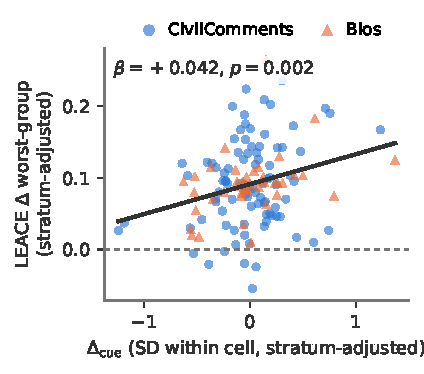
\includegraphics[width=0.94\columnwidth]{fig_target.pdf}
\caption{\textbf{Cue reliance provides signal for erasure gains.}
Partial-regression view of the first row of Table~\ref{tab:target}, showing
LEACE worst-group gain against \cued{} with both adjusted for
cell$\times\rho$ stratum ($n{=}135$). In this specification, higher \cued{}
is associated with larger gain.}
\label{fig:target}
\end{figure}

\begin{table}[t]
\centering\small
\begin{tabular}{llrr}
\toprule
\cued{} standardized & baseline ctrl & $\beta$ & $p$ \\
\midrule
within cell    & no  & $+.0417$ & $.0018$ \\
within cell    & yes & $+.0337$ & $.0060$ \\
within stratum & no  & $+.0125$ & $.0134$ \\
within stratum & yes & $+.0086$ & $.0657$ \\
\bottomrule
\end{tabular}
\caption{\textbf{\cued{} provides repair-targeting signal in three of four
specifications.} Post-LEACE worst-group gain regressed on \cued{}. All rows
include cell$\times\rho$ (stratum) fixed effects, $n{=}135$.}
\label{tab:target}
\end{table}

\section{What Exact Control of $\rho$ Reveals}
\label{sec:exact}

\begin{figure}[t]
\centering
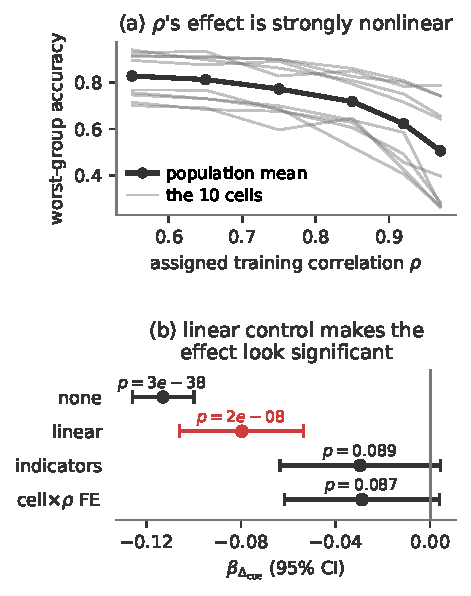
\includegraphics[width=0.9\columnwidth]{fig_trap.pdf}
\caption{\textbf{Why linear control of $\rho$ is unreliable.} (a)~The effect of $\rho$ on worst-group accuracy is flat at low $\rho$ and steep at high $\rho$ ($F(4,165){=}13.4$). (b)~The \cued{} coefficient under four controls for $\rho$. Its apparent significance under linear control disappears under exact control.}
\label{fig:trap}
\end{figure}

\paragraph{A pitfall of linear control.}
Our own first analysis, mirroring common practice, entered $\rho$ linearly and
made \cued{} appear strongly predictive beyond the assigned training
correlation. But $\rho$'s
effect is strongly nonlinear
($F(4,165){=}13.4$, $p{=}1.7{\times}10^{-9}$, Fig.~\ref{fig:trap}a). Linear control therefore leaves residual $\rho$ variance that any correlated measurement can absorb. This is the classic residual-confounding problem \citep{groenwold2013adjustment}. Table~\ref{tab:ladder} and Fig.~\ref{fig:trap}b show the pattern. The coefficient is significant under no control and under
linear control, but not under indicators.
With a discrete assigned factor, saturated adjustment uses four additional
degrees of freedom \citep{lin2013agnostic}. A linearly misspecified control, by
contrast, can bias the coefficient of interest more than omitting the control
entirely \citep{goff2014linear}. For this discrete assigned factor, we avoid a linear specification. The population-of-models literature contains both practices today.
\citet{jiang2020fantastic} condition exactly and compute rank correlations
within fixed settings of every other design factor. More recent work in the
same genre controls its design grid with partial correlations on residuals
\citep{tan2024fractal}. 


\paragraph{The within-recipe estimate.}
At fixed recipe, the signal is much weaker. The pre-specified equal-weighted
estimator is negative and nominally significant ($p{=}.012$), but the result is
not robust. A permutation test gives $p{=}.061$. Leave-one-cell-out checks range from
$p{=}.033$ to $p{=}.079$, so the result is sensitive to which cell is removed.
The pre-specified confirmation half gives $p{=}.141$. We therefore do not treat
random-seed ranking within a fixed recipe as established.

The direction is nevertheless fairly consistent across strata. A conservative
equivalence analysis rules out only effects larger than about $14\%$ of the
between-correlation effect, so the data also do not support a tight equivalence
claim. Fixed-recipe differences therefore carry a small and statistically fragile signal. Most of \cued{}'s predictive power comes from placing models
across training-correlation levels without observing the assigned correlation.

\paragraph{``Used'' vs.\ ``decodable,'' scoped.}
Across training-correlation levels, \cued{} predicts worst-group accuracy
better than a linear probe for the cue. At fixed recipe, neither provides a
robust ranking signal, and the probe is near ceiling. The comparison therefore
supports the across-correlation result but is uninformative for seed-level
ranking.

\section{Cue Discovery and Label Efficiency}
\label{sec:extras}

We close with two practical properties of the audit, cue discovery and label
efficiency.

\paragraph{Automatic cue discovery.}
So far the audit assumes that the suspected cue is known. On CivilComments, we
test how much this requirement can be relaxed. We replace the oracle lexicon with the top-20 PMI tokens from each model's own
training draw, using add-100 smoothing \citep{gururangan2018artifacts}. The
discovered cue sets overlap the oracle by only $1.4/20$ words on average, yet
reliance measured with them still predicts worst-group accuracy
($r=-0.55/-0.60/-0.63$ across civil cells). So the result does not depend on
the hand-written lexicon. Cue discovery does, however, use the model's training draw, which the audit itself does not.

\paragraph{Label efficiency.}
A second practical advantage is that \cued{} does not require group-labeled
evaluation data. Using only 25 unlabeled cue-containing texts, it matches or
beats an estimate based on 10 group-labeled examples per group in five of six
cells. Direct group labels remain more useful in CivilComments, while on two
Bios cells \cued{} remains competitive even with substantially larger labeled
sets. Appendix~\ref{app:label} gives the full comparison. Appendix~\ref{app:ew} reports a related negative result on using early-training
\cued{} as an early-warning signal.


\section{Discussion}

Studies of this kind often explain model performance using the design factors
that generated the model population
\citep{morris2019simulation,jiang2020fantastic}. Our results offer a complementary view. At held-out training-correlation levels, measuring the
finished model can be more informative than simple extrapolation from the
assigned correlation. The training correlation still matters, but its effect on worst-group accuracy is strongly nonlinear. Simple extrapolation can therefore fail, while
\cued{} measures the reliance the trained model actually expresses. Combined with the repair results, this provides a concrete
example of actionable interpretability \citep{orgad2026actionable}. The measurement predicts a downstream failure and informs the choice of which models to repair. Exact control also clarifies the scope of the result.
Most of \cued{}'s predictive power is across correlation levels, while the
relationship within a fixed recipe is small and not robust.


\section{Conclusion}

This paper asked whether counterfactual cue reliance can serve as an
actionable audit of a finished model. In the controlled populations we trained, the answer is yes, within a scope we can state precisely. Higher \cued{} predicts
lower worst-group accuracy. In a separate high-seed analysis, the prediction
carries over to held-out training-correlation levels, where simple
extrapolation from the assigned correlation performs poorly. \cued{} also gives a useful signal for choosing which models to repair with LEACE. Exact control sets the scope. Most of the predictive signal is across correlation levels,
and differences across random seeds within a fixed recipe are small and
statistically fragile. For a practitioner with a fine-tuned classifier and a
suspected cue, the lesson is simple. In these settings, what the finished
model does with the cue tells you more about shortcut failure than
extrapolating from the correlation it was trained on.

\noindent Supplementary code is available at:\\
\url{https://github.com/prakharg55/cue_reliance}.

\section*{Limitations}

\paragraph{Scope and generalization.}
We study two English binary-classification tasks, decoder LMs of
0.4--1.5B parameters, and lexical cues. Structural or distributed cues are
outside our scope. The result also does not extend directly to heterogeneous public checkpoints. Across eight public toxicity classifiers, capability
dominated and \cued{} was not predictive ($r{=}{+}0.06$). Whether reliance
can be separated from capability across uncontrolled models remains open. The audit is label-free, but it still assumes a candidate cue and a meaningful counterfactual edit. Whether the result holds for substantially
larger instruction-tuned models is untested.

\paragraph{Prediction limits.}
At fixed $\rho$, the relationship across random seeds is small and not
robustly established (permutation $p{=}.061$, confirmation-half $p{=}.141$).
The out-of-regime analysis tests only linear and nearest-level extrapolation
from two observed $\rho$ levels. With only two observed levels per fold, any nonlinear extrapolation requires an assumed shape that the data cannot determine. Stronger theory-motivated recipe predictors remain an open comparison. Alternative perturbation or attribution summaries also remain
untested. Our probe baseline measures cue decodability. It does not measure task--cue direction entanglement.

\paragraph{Repair limits.}
Our DFR implementation refits on training data and may therefore overstate
its performance. Repair targeting misses significance in its strictest
specification ($p{=}.066$), and part of its signal overlaps with baseline
headroom. Mediation-style decompositions of the $\rho$ effect were unstable
at our sample size and are not reported.




\section*{Ethics Statement}

Both datasets are standard, publicly released research corpora, namely
CivilComments (CC0) and Bias-in-Bios. The identity lexicon deliberately excludes ambiguous
terms (e.g., \emph{white}, \emph{black}) that are unreliable identity
references. We do not infer demographic attributes of any person, and we
perform no dialect inference. Toxic example texts appear only in aggregate
statistics. The $\rho$-controlled populations intentionally train models with
amplified spurious behavior. All such models exist only as measurement logs,
and none is released. \cued{} is an audit measurement. We caution against interpreting low \cued{} alone as certification of fairness, especially since it did not separate from capability on uncontrolled public models.

\section*{Acknowledgments}
This material is based in part upon work supported
by the German Federal Ministry of Education and Research (BMBF): Tübingen AI Center, FKZ: 01IS18039B; by the Machine Learning Cluster of Excellence, EXC number 2064/1 – Project number 390727645; % if Zhijing has the MPI or Tuebingen affiliation
% by NSERC Discovery Grant RGPIN-2025-06491; % for causality research
% by the University of Toronto’s Acceleration Consortium, which receives funding from the Canada First Research Excellence Fund (CFREF); % causality; also AI for science work
% by the Frontier Model Forum and AI Safety Fund; % for multi-agent and sanctioning research
by Coefficient Giving; % if the work is general AI safety-related
by Schmidt Sciences; % if the worker is on the topic of Mech Interp or test data contamination
% by the Canadian AI Safety Institute Research Program at CIFAR through a Catalyst Award; % multicultural awareness for LLMs
% by the Survival and Flourishing Fund; % democraccy work
by the Cooperative AI Foundation; by the Canadian AI Safety Institute Research Program at CIFAR. % for multi agent research
Resources used in preparing this research project were provided, in part, by the Digital Research Alliance of Canada; the Province of Ontario; the Swiss AI Compute grants; the Government of Canada through CIFAR; and companies sponsoring the Vector Institute.
F.D. acknowledges support through a fellowship from the Hector Fellow Academy.
We thank Jiarui Liu, Andrew Kim, and the other key developers of PaperMentor \citep{liu2026papermentorhumancenteredmultiagentwriting}, which provides mentorship and valuable suggestions in polishing this paper after the first draft by the authors. We further acknowledge the crucial work of AdminBot for administrative support that streamlined our research workflow.

\bibliography{references}

\appendix

\section{Reproducibility and Verification}
\label{app:repro}
All numbers in this paper are produced by analysis scripts from raw training
logs and re-verified mechanically. A checker traces every reported value,
including the tables in this appendix, to regenerated script output, and the
figures assert their plotted values against the same captured results. The
pre-specified primary analysis of \S\ref{sec:exact} was locked before the
confirmation half of the high-seed data was analyzed. Trained weights were
not retained, so re-analysis of the models themselves requires retraining
from the configuration in Appendix~\ref{app:config}. The training code, the
analysis code and the logs of all trained models are in the repository linked
in the Conclusion.

\section{Experimental Detail}
\label{app:setup}
This section records the training configuration and the data-side audits
behind \S\ref{sec:design}.

Across study arms, the frozen $2{\times}2{\times}2$ grid contains 144 models,
the three-family grid contains 108, and the high-seed arm adds 108 new models.
The robustness arms contain 36 models from Qwen-civil under full fine-tuning
and an instruction-tuned base. The per-epoch trajectories contain 72 models
from Qwen-civil and Pythia-civil, and the placebo arm contains 18 models from
Qwen-civil. This gives 486 trained models in total. All runs completed.

\subsection{Training Configuration}
\label{app:config}
All models are decoder LMs fine-tuned as binary classifiers scored by the
logit difference of the two answer tokens at the last position. LoRA:
$r{=}16$, $\alpha{=}32$, dropout $0.05$, applied to all attention and MLP
projections. Optimization: AdamW, lr $2{\times}10^{-4}$, 4 epochs, batch 32
(civil) and 24 (bios), $n_{\text{train}}{=}4{,}000$, max length 96 (civil)
and 160 (bios) tokens, fp32. The full fine-tuning arm uses lr
$2{\times}10^{-5}$ with no adapter. The instruction-tuned arm uses the same
recipe on an instruct base. Families: Qwen2.5 (0.5B, 1.5B), Pythia (410m,
1.4b), OLMo-2 (1B). \cued{} is estimated on 300 held-out texts that contain
the cue per model.

Base checkpoints are Qwen2.5-0.5B, Qwen2.5-1.5B, and Qwen2.5-0.5B-Instruct,
Pythia-410m and Pythia-1.4b, and OLMo-2-0425-1B, all from the Hugging Face
Hub under the \texttt{Qwen}, \texttt{EleutherAI}, and
\texttt{allenai} organizations. Each run used a single NVIDIA A100 GPU. The
490 scheduler jobs behind the reported results, covering the 486 fine-tuning
runs and the public-classifier evaluations, total 83 GPU-hours, with a median
of 7.5 minutes per job. Software: PyTorch 2.9.0, PEFT 0.19.1, scikit-learn
1.6.1, and statsmodels 0.14.2. The Transformers version used at training time
was not recorded.

\subsection{Counterfactual Edit Audit}
\label{app:edits}
We audited the realized correlations of actual training draws, re-detecting cue presence from the text itself instead of from the sampling key. At $\rho{=}0.55$ the realized
$P(\text{toxic}\mid\text{cue})$ and $P(\text{toxic}\mid\text{no cue})$ are
$0.550$ and $0.450$, at $\rho{=}0.97$ they are $0.970$ and $0.030$, and label
balance is $0.500$ in both audited draws.

Civil (identity term $\rightarrow$ ``people''): held-out group sizes
796--800 per group, 1{,}598 eval texts that contain the cue, $100.0\%$
changed by the edit, mean $1.50$ tokens replaced per text (median 1, max 10),
mean text length 49 words, edit fraction $3.1\%$ of tokens.

Bios (labels professor vs.\ physician, male$\rightarrow$female lexicon swap):
group sizes 800 per group, 1{,}600 male-cue eval texts, $99.9\%$ changed,
mean $3.14$ tokens swapped (median 3, max 10), mean length 60 words, edit
fraction $5.2\%$. The swap does not undo itself. Applying it twice changes
$67.4\%$ of texts, because his and him both map to her and the reverse map
returns his. The measurement therefore uses only the well-defined
male$\rightarrow$female direction.

\subsection{Cue and Placebo Lexicons}
\label{app:lexicons}
Identity lexicon (32 terms): arab, asian, atheist, bisexual, buddhist,
catholic, christian, christianity, christians, feminist, gay, gays, hindu,
hispanic, homosexual, immigrant, islam, islamic, jew, jewish, jews, latina,
latino, lesbian, lgbt, lgbtq, mexican, mormon, muslim, muslims, queer,
transgender. Ambiguous terms (e.g., white, black, american) are deliberately
excluded as unreliable identity references.

Placebo lexicon (32 words, matched to the identity lexicon's per-word
document-frequency profile on the 16{,}000-text training pool, total
document frequency 10{,}151 vs.\ 10{,}184, screened to exclude identity
content): attacking, believes, chose, court, damn, damned, deal, doctrines,
having, heard, idea, know, laws, long, maher, makes, meaningless, member,
movie, needs, oregon, paid, perhaps, right, sanders, should, sure, take,
think, want, west, years.

In the placebo arm, shifts are $17.8\times$ smaller after adjustment for edit
coverage and are weakly correlated with \cued{} ($r{=}{-}0.11$).
The placebo--worst-group correlation is $+0.08$ ($p{=}0.75$), compared with
$-0.905$ ($p{=}2.4{\times}10^{-7}$) for the cue edit.

\section{Statistical Detail for the Population Results}
\label{app:stats}
This section gives the exact values behind the estimates of
\S\ref{sec:prediction} and \S\ref{sec:exact}.

\subsection{Extrapolation and Ladder Estimates}
\label{app:tables}
Tables~\ref{tab:oor} and \ref{tab:ladder} give the exact values behind
Fig.~\ref{fig:hero}b and Fig.~\ref{fig:trap}b, including the nearest-level
step baseline quoted in \S\ref{sec:prediction}.

\begin{table}[t]
\centering\small
\begin{tabular}{lcc}
\toprule
predictor & $R^2$ & MAE \\
\midrule
\cued{} (measured on the model) & $+0.571$ & $0.127$ \\
$\rho$ (assigned correlation)    & $-0.182$ & $0.219$ \\
nearest-level step (from $\rho$) & $-0.140$ & $0.220$ \\
linear probe (decodability)     & $+0.037$ & $0.186$ \\
\bottomrule
\end{tabular}
\caption{\textbf{The model-side measurement extrapolates better than the
assigned correlation.}
Leave-one-$\rho$-out evaluation, fitting on two correlation levels and
predicting the held-out models at the third (cell fixed effects, $n{=}135$).
The step baseline predicts each held-out model with its cell's nearest
observed level.}
\label{tab:oor}
\end{table}

\begin{table}[t]
\centering\small
\begin{tabular}{lrr}
\toprule
control for $\rho$ & $\beta_{\cued}$ & $p$ \\
\midrule
none              & $-.1129$ & $3.1{\times}10^{-38}$ \\
linear            & $-.0796$ & $1.6{\times}10^{-8}$ \\
indicators        & $-.0296$ & $.089$ \\
cell$\times\rho$ FE & $-.0288$ & $.087$ \\
\bottomrule
\end{tabular}
\caption{\textbf{Linear control overstates the apparent effect of \cued{}.}
The same regression under four controls for $\rho$ ($n{=}180$, cell fixed
effects throughout). The apparent significance after linear control disappears
under exact control.}
\label{tab:ladder}
\end{table}

\subsection{Per-Stratum Detail}
\label{app:strata}
Table~\ref{tab:strata} gives the nine within-stratum regressions behind the
pre-specified estimate of \S\ref{sec:exact}, and Table~\ref{tab:standard}
the same effect under all four scaling choices. The estimate is strongest
when both variables are standardized within stratum ($p{=}.015$) and weakest
under the mismatched scaling, z within cell with stratum fixed effects
($p{=}.147$). The equivalence bound in Appendix~\ref{app:tost} deliberately
uses that widest interval.

The pre-specified equal-weighted estimator is $-0.027$ accuracy points per
\cued{} unit ($t(8){=}{-}3.26$, $p{=}.012$). Across the nine strata, the pooled
correlation is $-0.224$ (95\% CI $[-0.394,-0.039]$), with
$Q(8){=}4.5$ and $I^2{=}0\%$. Seven of nine slopes are negative, with both
positive slopes at $\rho{=}0.97$. The spread of \cued{} increases from about
$0.26$ at $\rho{=}0.65$ to $1.30$ at $\rho{=}0.97$, causing pooled
fixed-effects OLS to place $76\%$ of its weight on the $\rho{=}0.97$ strata and
$3\%$ on $\rho{=}0.65$. Robustness checks give permutation $p{=}.061$ and leave-one-cell-out
$p{=}.038/.079/.033$ when dropping Pythia-civil, Qwen-bios, and Qwen-civil,
respectively. The confirmation half gives $p{=}.141$ on the pre-specified
seeds 9--14.

For the probe comparison, probe partial effects are null in 7 of 8 frozen
cells. Within fixed strata, probe SD is $0.0007$--$0.0156$, compared with
$0.24$--$1.70$ for \cued{}, explaining why the fixed-recipe probe comparison
is largely ceiling-limited.

\begin{table}[t]
\centering\small
\setlength{\tabcolsep}{4.5pt}
\begin{tabular}{llrrrr}
\toprule
cell & $\rho$ & SD(\cued) & SD($w$) & $b$ & $r$ \\
\midrule
Pythia-civil & .65 & 0.249 & .085 & $-.042$ & $-.123$ \\
Pythia-civil & .85 & 0.452 & .105 & $-.054$ & $-.233$ \\
Pythia-civil & .97 & 0.966 & .087 & $+.010$ & $+.107$ \\
Qwen-bios    & .65 & 0.236 & .029 & $-.039$ & $-.318$ \\
Qwen-bios    & .85 & 0.948 & .037 & $-.016$ & $-.405$ \\
Qwen-bios    & .97 & 1.703 & .094 & $-.023$ & $-.413$ \\
Qwen-civil   & .65 & 0.297 & .041 & $-.059$ & $-.428$ \\
Qwen-civil   & .85 & 0.592 & .057 & $-.023$ & $-.233$ \\
Qwen-civil   & .97 & 1.224 & .084 & $+.007$ & $+.097$ \\
\bottomrule
\end{tabular}
\caption{Within-stratum slopes ($b$, raw accuracy points per \cued{} unit)
and correlations ($r$), 15 seeds per stratum. SD($w$) is the within-stratum
SD of worst-group accuracy.}
\label{tab:strata}
\end{table}

\begin{table}[t]
\centering\small
\setlength{\tabcolsep}{4.5pt}
\begin{tabular}{lrr}
\toprule
specification & $\beta$ & $p$ \\
\midrule
z within cell + stratum FE (mismatched) & $-.0254$ & $.147$ \\
z within stratum + stratum FE           & $-.0124$ & $.060$ \\
raw \cued{} + stratum FE                & $-.0129$ & $.084$ \\
both z within stratum                   & $-.2166$ & $.015$ \\
\bottomrule
\end{tabular}
\caption{The same within-recipe effect under four combinations of predictor
scaling and fixed effects ($n{=}135$). The first row is the most
conservative and is the interval used for the equivalence bound.}
\label{tab:standard}
\end{table}

\subsection{Equivalence Bounds}
\label{app:tost}
The bounded interval is the 90\% CI of the pooled regression of worst-group
accuracy on within-cell-standardized \cued{} with stratum fixed effects, the
widest and therefore most conservative of the four scalings in
Table~\ref{tab:standard}. Scale anchors: within-stratum SD of worst-group
accuracy $0.0737$, and the between-correlation effect ($\rho\,0.97$ vs.\ $0.65$)
$-0.3875$ accuracy points.
Following \citet{braun2022equivalence} we report the TOST verdict across
margins (Table~\ref{tab:tost}) rather than a single chosen margin. Principled
candidate margins span $0.007$ (a tenth of the within-stratum SD) to $0.039$
(a tenth of the between-correlation effect), and none of them supports an equivalence
claim.

\begin{table}[t]
\centering\small
\begin{tabular}{rrrl}
\toprule
margin & \% of $\rho$ effect & TOST $p$ & verdict \\
\midrule
.020 &  5.2 & .622 & not equivalent \\
.030 &  7.7 & .396 & not equivalent \\
.040 & 10.3 & .202 & not equivalent \\
.050 & 12.9 & .080 & not equivalent \\
.054 & 14.0 & .050 & boundary \\
.060 & 15.5 & .025 & equivalent \\
.075 & 19.4 & .003 & equivalent \\
.100 & 25.8 & .000 & equivalent \\
\bottomrule
\end{tabular}
\caption{TOST margin sensitivity for the within-recipe effect. ``Equivalent''
means effects larger than the margin are rejected at $\alpha{=}.05$.}
\label{tab:tost}
\end{table}

\section{Repair Detail}
\label{app:repairdetail}
This section supports \S\ref{sec:repair} with the overall-accuracy cost of
each repair and the budgeted allocation experiment.

\paragraph{Intervention layers.}
LEACE and the fixed-depth ablation act at layer
$\mathrm{round}(20\,n_{\text{layers}}/24)$, which is layer 20 in the 24-layer
models and the same relative depth otherwise. The LEACE eraser and the
ablation directions are fit on training-split texts only. The prospective arm
instead selects, from training-side texts alone, the layer whose direction
projection most reduces training-side \cued{}.

\subsection{Overall-Accuracy Cost}
\label{app:repaircost}
Table~\ref{tab:repaircost} reports mean post-repair overall accuracy next to
the worst-group gains of Table~\ref{tab:repair}. Post-LEACE overall accuracy
is within $0.03$ of DFR's in every cell. The two cells where hard ablation is strongly harmful for worst-group
accuracy also show large overall-accuracy losses.

\begin{table}[t]
\centering\small
\setlength{\tabcolsep}{4.2pt}
\begin{tabular}{lrrrr}
\toprule
cell & ablate & LEACE & DFR & AFR \\
\midrule
Qwen-civil   & .771 & .762 & .782 & .755 \\
Pythia-civil & .627 & .772 & .790 & .775 \\
OLMo-civil   & .686 & .790 & .807 & .785 \\
Qwen-bios    & .938 & .937 & .948 & .931 \\
Pythia-bios  & .926 & .934 & .949 & .927 \\
OLMo-bios    & .949 & .946 & .957 & .940 \\
\bottomrule
\end{tabular}
\caption{Mean post-repair overall accuracy ($n{=}18$/cell). Post-repair
overall accuracy was not logged for the prospectively-selected-layer arm.}
\label{tab:repaircost}
\end{table}

\subsection{Allocation Under a Budget}
\label{app:alloc}
Each high-seed cell (45 models) is evaluated independently, with each
policy's ranking rule fixed in advance, so nothing is fitted. Policies rank
by descending \cued{} (within-cell standardized), by headroom ($1-$baseline
worst, identical to ranking by visible failure), by assigned $\rho$
(stratum-mean expectation, since $\rho$ cannot rank within a stratum), or by
realized gain (oracle). Repairing the top 15: random $+0.091$, \cued{}
$+0.200$, headroom $+0.201$, highest-$\rho$ $+0.201$, oracle $+0.205$
(per-cell \cued{} selections $+0.303/+0.116/+0.182$ against oracle
$+0.307/+0.118/+0.189$). At this budget, selection is chiefly correlation-level identification, consistent with the fragile fixed-recipe effect
(\S\ref{sec:exact}).

Table~\ref{tab:sweep} reports the full budget sweep. At budgets below one
stratum the measurement ranks within the high-$\rho$ stratum, which $\rho$
cannot, and the \cued{} selection is far outside what random selection
attains. Across the three cells, the probability that a random subset matches
it is at most $0.014$ at budget 5 and below $10^{-4}$ at budget 10 (10{,}000
draws per cell). Headroom itself correlates with gain at $r{=}0.79$, the
confound reported in \S\ref{sec:repair}.

\begin{table}[t]
\centering\small
\begin{tabular}{rrrrrr}
\toprule
budget & random & \cued{} & headroom & $\rho$ & oracle \\
\midrule
 5 & .091 & .224 & .218 & .201 & .281 \\
10 & .091 & .214 & .210 & .201 & .237 \\
15 & .091 & .200 & .201 & .201 & .205 \\
20 & .091 & .173 & .176 & .170 & .181 \\
30 & .091 & .138 & .139 & .138 & .142 \\
\bottomrule
\end{tabular}
\caption{Mean realized LEACE gain of the selected models by repair budget
(of 45 per cell, averaged over the three cells). The $\rho$ policy uses
stratum-mean expectations, since $\rho$ cannot rank within a stratum.}
\label{tab:sweep}
\end{table}

\section{Additional Analyses}
\label{app:additional}
This section collects the secondary analyses referenced from the main text.

\subsection{Label-Efficiency Detail}
\label{app:label}
Table~\ref{tab:label} gives the correlation between each estimator and true
worst-group accuracy across the 18 models of each cell. It compares direct
estimation from $k$ group-labeled examples per group, which also requires the
roughly 4{,}000 labels behind the group split, against \cued{} from $m$
unlabeled texts that contain the cue.

\begin{table}[t]
\centering\small
\setlength{\tabcolsep}{3.6pt}
\begin{tabular}{lrrrrrrr}
\toprule
 & \multicolumn{4}{c}{labeled, $k$/group} & \multicolumn{3}{c}{\cued{}, $m$ unlabeled} \\
\cmidrule(lr){2-5}\cmidrule(lr){6-8}
cell & 5 & 10 & 25 & 50 & 25 & 100 & 300 \\
\midrule
Qwen-civil   & .70 & .83 & .92 & .96 & .87 & .90 & .91 \\
Pythia-civil & .68 & .82 & .92 & .96 & .72 & .76 & .77 \\
OLMo-civil   & .63 & .78 & .90 & .95 & .84 & .89 & .90 \\
Qwen-bios    & .34 & .51 & .72 & .84 & .92 & .93 & .93 \\
Pythia-bios  & .58 & .75 & .87 & .94 & .81 & .81 & .81 \\
OLMo-bios    & .37 & .53 & .73 & .86 & .87 & .88 & .88 \\
\bottomrule
\end{tabular}
\caption{Correlation with true worst-group accuracy per cell ($n{=}18$
models each).}
\label{tab:label}
\end{table}

\subsection{Early Measurability}
\label{app:ew}
\cued{} measured after one of four training epochs already correlates
$-0.886$ with final worst-group accuracy, and the epoch-1 signal keeps
$108.4\%$ of the final measurement's $R^2$ ($0.785/0.724$). It is not,
however, a useful early-warning tool. Epoch-1 overall accuracy predicts final worst-group accuracy equally well ($r{=}{+}0.875$). After cell fixed effects and exact $\rho$ control, no epoch-1 signal, including \cued{}, adds predictive value ($\Delta R^2{=}0.000$, $p{=}0.65$), because within a stratum
the epoch-1 signals share their variance. Table~\ref{tab:ew} lists all
predictors.

\begin{table}[t]
\centering\small
\setlength{\tabcolsep}{4.5pt}
\begin{tabular}{lrrr}
\toprule
epoch-1 predictor & $r$ & ctrl.\ $\beta$ & ctrl.\ $p$ \\
\midrule
\cued{}                    & $-.886$ & $+.013$ & $.669$ \\
final \cued{} (ceiling)    & $-.851$ & $-.012$ & $.327$ \\
worst-group (oracle)       & $+.836$ & $-.049$ & $.621$ \\
worst-class (label-free)   & $+.710$ & $-.048$ & $.735$ \\
overall accuracy           & $+.875$ & $+.019$ & $.950$ \\
train loss                 & $+.811$ & $+.115$ & $.742$ \\
\bottomrule
\end{tabular}
\caption{Epoch-1 predictors of final worst-group accuracy
($n{=}72$, Qwen-civil and Pythia-civil). Raw correlations are uniformly
strong. Under cell fixed effects and exact $\rho$ control, none survives.}
\label{tab:ew}
\end{table}

\subsection{The Unused Instrument}
\label{app:iv}
Because $\rho$ is randomized, it is formally available as an instrument for
\cued{}. On the high-seed sample the first stage is strong by construction
($+15.0$ \cued{} units per unit $\rho$), and two-stage least squares gives
$-0.077$ against an OLS estimate of $-0.062$ (ratio $1.24$, cell fixed
effects). We do not interpret this coefficient causally because the exclusion
restriction, that $\rho$ affects worst-group accuracy only through \cued{}, is
likely violated. We therefore report it only as a descriptive sensitivity
analysis.

\subsection{The Public-Classifier Arm}
\label{app:public}
Table~\ref{tab:public} evaluates eight off-the-shelf toxicity classifiers
under the same protocol as the main study (same held-out split, same edit,
train-side threshold calibration, toxic-logit scoring for multi-label heads).
Worst-group accuracy tracks overall accuracy almost perfectly
(Spearman $+0.98$), and \cued{} does not predict worst-group accuracy
($r{=}{+}0.06$, $p{=}0.88$). This is the scope limit reported in
Limitations. In this small heterogeneous set, capability differences dominate, and \cued{}
does not separate from them.

\begin{table}[t]
\centering\small
\setlength{\tabcolsep}{4.5pt}
\begin{tabular}{lrrr}
\toprule
model & worst & overall & \cued{} \\
\midrule
s-nlp/roberta\_toxicity          & .838 & .894 & $+2.28$ \\
martin-ha/toxic-comment          & .807 & .854 & $+0.86$ \\
unitary/toxic-bert               & .790 & .846 & $+0.81$ \\
JungleLee/bert-toxic             & .735 & .828 & $+1.04$ \\
cardiffnlp/twitter-offensive     & .662 & .799 & $+0.12$ \\
CNERG/dehatebert-mono-en         & .580 & .667 & $+0.26$ \\
citizenlab/distilbert-toxicity   & .565 & .726 & $-0.04$ \\
facebook/dynabench-r4            & .330 & .626 & $+1.86$ \\
\bottomrule
\end{tabular}
\caption{Public classifiers under the study protocol, sorted by worst-group
accuracy. Capability ordering and worst-group ordering nearly coincide.}
\label{tab:public}
\end{table}

\end{document}
